\documentclass {article}
\usepackage[utf8]{inputenc}
\usepackage {tabto}
\usepackage {enumitem}
\usepackage {graphicx}
\begin {document}
\section {Calculus}      
\begin {enumerate}
\item A rectangular visiting card is to contain $24\,sq.cm$ of printed matter. The margins at the top and bottom of the card are to be $1\,cm$ and the margins on the left and right are to be $1 \frac{1}{2}cm$ as shown below :
        \begin {figure} [h!]
        \centering
        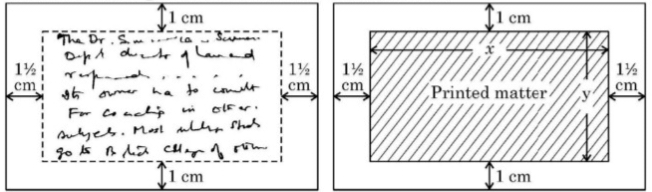
\includegraphics[width=0.8\textwidth] {/storage/emulated/0/DCIM/Screenshots/figure2.jpg}
        \end {figure}
\\On the basis of the above information, answer the following questons:
        \begin {enumerate}
\item [(i)] Write the expression for the area of the visiting card in terms of x.
\item [(ii)] Obtain the dimensions of the card of minimum area.
        \end {enumerate}
\end {enumerate}
\end {document}
~
